\documentclass[aspectratio=169, xcolor=dvipsnames]{beamer}

% --- Theme Setup ---
\usetheme{Madrid}
\usecolortheme{default}

% --- Packages ---
\usepackage{graphicx}
\usepackage{xcolor}
\usepackage{booktabs}
\usepackage{hyperref}
\usepackage{adjustbox}
\usepackage{amssymb}
\usepackage{amsmath}
\usepackage{listings}
\usepackage{caption}

\lstset{
  basicstyle=\ttfamily\small,
  keywordstyle=\color{blue}\bfseries,
  stringstyle=\color{red},
  showstringspaces=false,
  breaklines=true
}

% --- Title Information ---
\title{Module 17}
\subtitle{Formal Relational Query Languages/2}
\author{Milav Dabgar}
\institute{www.milav.in}
\date{\today}

\begin{document}

% Title Slide
\begin{frame}
    \titlepage
\end{frame}

\begin{frame}{Module Recap}
    \begin{itemize}
        \item Relational Algebras and its Operations
    \end{itemize}
\end{frame}

\begin{frame}{Module Objectives}
    \begin{itemize}
        \item To understand formal calculus-based query language through relational algebra
    \end{itemize}
\end{frame}

\begin{frame}{Module Outline}
    \begin{itemize}
        \item Tuple Relational Calculus (Overview only)
        \item Domain Relational Calculus (Overview only)
        \item Equivalence of Algebra and Calculus
    \end{itemize}
\end{frame}

\begin{frame}{Formal Relational Query Language}
    \begin{itemize}
        \item Relational Algebra
        \begin{itemize}
            \item Procedural and Algebra based
        \end{itemize}
        \item Tuple Relational Calculus
        \begin{itemize}
            \item Non-Procedural and Predicate Calculus based
        \end{itemize}
        \item Domain Relational Calculus
        \begin{itemize}
            \item Non-Procedural and Predicate Calculus based
        \end{itemize}
    \end{itemize}
\end{frame}

\section{Predicate Logic}
\begin{frame}
  \vfill
  \centering
  \begin{beamercolorbox}[sep=8pt,center,shadow=true,rounded=true]{title}
    \usebeamerfont{title}Predicate Logic\par%
  \end{beamercolorbox}
  \vfill
\end{frame}

\begin{frame}{Predicate Logic}
    \begin{itemize}
        \item Predicate Logic or Predicate Calculus is an extension of Propositional Logic or Boolean Algebra.
        \item It adds the concept of predicates and quantifiers to better capture the meaning of statements that cannot be adequately expressed by propositional logic.
        \item Tuple Relational Calculus and Domain Relational Calculus are based on Predicate Calculus.
    \end{itemize}
\end{frame}

\begin{frame}{Predicate}
    \begin{itemize}
        \item Consider the statement, '$x$ is greater than 3'. It has two parts. The first part, the variable $x$, is the subject of the statement. The second part, 'is greater than 3', is the predicate. It refers to a property that the subject of the statement can have.
        \item The statement '$x$ is greater than 3' can be denoted by $P(x)$ where $P$ denotes the predicate 'is greater than 3' and $x$ is the variable.
        \item The predicate $P$ can be considered as a function. It tells the truth value of the statement $P(x)$ at $x$. Once a value has been assigned to the variable $x$, the statement $P(x)$ becomes a proposition and has a truth or false value.
        \item In general, a statement involving $n$ variables $x_1, x_2, x_3, \dots, x_n$ can be denoted by $P(x_1, x_2, x_3, \dots, x_n)$. Here $P$ is also referred to as $n$-place predicate or a $n$-ary predicate.
    \end{itemize}
\end{frame}

\begin{frame}{Quantifiers}
    In predicate logic, predicates are used alongside quantifiers to express the extent to which a predicate is true over a range of elements. Using quantifiers to create such propositions is called quantification. There are two types of quantifiers:
    \begin{itemize}
        \item Universal Quantifier
        \item Existential Quantifier
    \end{itemize}
\end{frame}

\begin{frame}{Universal Quantifier}
    Universal Quantification: Mathematical statements sometimes assert that a property is true for all the values of a variable in a particular domain, called the domain of discourse.
    \begin{itemize}
        \item Such a statement is expressed using universal quantification.
        \item The universal quantification of $P(x)$ for a particular domain is the proposition that asserts that $P(x)$ is true for all values of $x$ in this domain.
        \item The domain is very important here since it decides the possible values of $x$.
        \item Formally, The universal quantification of $P(x)$ is the statement '$P(x)$ for all values of $x$ in the domain'.
        \item The notation $\forall P(x)$ denotes the universal quantification of $P(x)$. Here $\forall$ is called the universal quantifier. $\forall P(x)$ is read as 'for all $x$ $P(x)$'.
        \item Example: Let $P(x)$ be the statement '$x + 2 > x$'. What is the truth value of the statement $\forall x P(x)$?
        \item Solution: As $x + 2$ is greater than $x$ for any real number, so $P(x) \equiv T$ for all $x$ or $\forall x P(x) \equiv T$.
    \end{itemize}
\end{frame}

\begin{frame}{Existential Quantifier}
    Existential Quantification: Some mathematical statements assert that there is an element with a certain property. Such statements are expressed by existential quantification. Existential quantification can be used to form a proposition that is true if and only if $P(x)$ is true for at least one value of $x$ in the domain.
    \begin{itemize}
        \item Formally, the existential quantification of $P(x)$ is the statement 'There exists an element $x$ in the domain such that $P(x)$'.
        \item The notation $\exists P(x)$ denotes the existential quantification of $P(x)$. Here $\exists$ is called the existential quantifier. $\exists P(x)$ is read as 'There is atleast one such $x$ such that $P(x)$'.
        \item Example: Let $P(x)$ be the statement '$x > 5$'. What is the truth value of the statement $\exists x P(x)$?
        \item Solution: $P(x)$ is true for all real numbers greater than $5$ and false for all real numbers less than $5$. So $\exists x P(x) \equiv T$.
    \end{itemize}
\end{frame}

\section{Tuple Relational Calculus}
\begin{frame}
  \vfill
  \centering
  \begin{beamercolorbox}[sep=8pt,center,shadow=true,rounded=true]{title}
    \usebeamerfont{title}Tuple Relational Calculus\par%
  \end{beamercolorbox}
  \vfill
\end{frame}

\begin{frame}{Tuple Relational Calculus}
    TRC is a non-procedural query language, where each query is of the form
    \[ \{t \mid P(t)\} \]
    \begin{itemize}
        \item where $t =$ resulting tuples, $P(t) =$ known as predicate and these are the conditions that are used to fetch $t$. $P(t)$ may have various conditions logically combined with OR ($\lor$), AND ($\land$), NOT($\lnot$).
        \item It also uses quantifiers:
        \begin{itemize}
            \item $\exists t \in r (Q(t)) =$ 'there exists' a tuple in $t$ in relation $r$ such that predicate $Q(t)$ is true.
            \item $\forall t \in r (Q(t)) =$ $Q(t)$ is true 'for all' tuples in relation $r$.
        \end{itemize}
        \item $\{P \mid \exists S \in \text{Students and } (S.\text{CGPA} > 8 \land P.\text{name} = S.\text{sname} \land P.\text{age} = S.\text{age})\}$: returns the name and age of students with a CGPA above 8.
    \end{itemize}
\end{frame}

\begin{frame}{Predicate Calculus Formula}
    \begin{itemize}
        \item a) Set of attributes and constants
        \item b) Set of comparison operators: (e.g., $<, \leq, =, \neq, >, \geq$)
        \item c) Set of connectives: and ($\land$), or ($\lor$), not ($\lnot$)
        \item d) Implication ($\Rightarrow$): $x \Rightarrow y$, if $x$ is true, then $y$ is true. $x \Rightarrow y \equiv \lnot x \lor y$
        \item e) Set of quantifiers:
        \begin{itemize}
            \item $\exists t \in r (Q(t)) \equiv$ 'there exists' a tuple in $t$ in relation $r$ such that predicate $Q(t)$ is true
            \item $\forall t \in r (Q(t)) \equiv$ $Q$ is true 'for all' tuples $t$ in relation $r$
        \end{itemize}
    \end{itemize}
\end{frame}

\begin{frame}{TRC Example}
    \begin{center}
        \begin{adjustbox}{max width=0.6\textwidth}
        \begin{tabular}{|l|l|l|l|}
        \hline
        \textbf{Student Fname} & \textbf{Student Lname} & \textbf{Student Age} & \textbf{Student Course} \\ \hline
        David & Sharma & 27 & DBMS \\ \hline
        Aaron & Lilly & 17 & JAVA \\ \hline
        Sahil & Khan & 19 & Python \\ \hline
        Sachin & Rao & 20 & DBMS \\ \hline
        Varun & George & 23 & JAVA \\ \hline
        Simi & Verma & 22 & JAVA \\ \hline
        \end{tabular}
        \end{adjustbox}
    \end{center}
    Q.1 Obtain the first name of students whose age is greater than 21.
    
    \textbf{Solution:}
    \begin{itemize}
        \item $\{t.\text{Fname} \mid \text{Student}(t) \land t.\text{age} > 21\}$
        \item $\{t.\text{Fname} \mid t \in \text{Student} \land t.\text{age} > 21\}$
        \item $\{t \mid \exists s \in \text{Student} (s.\text{age} > 21 \land t.\text{Fname} = s.\text{Fname})\}$
    \end{itemize}
\end{frame}

\begin{frame}{TRC Example (2)}
    Consider the relational schema \texttt{student(rollNo, name, year, courseId)} and \texttt{course(courseId, cname, teacher)}
    \begin{itemize}
        \item Q.2 Find out the names of all students who have taken the course name 'DBMS'.
        \begin{itemize}
            \item $\{t \mid \exists s \in \text{student } \exists c \in \text{course } (s.\text{courseId} = c.\text{courseId} \land c.\text{cname} = '\text{DBMS}' \land t.\text{name} = s.\text{name})\}$
            \item $\{s.\text{name} \mid s \in \text{student} \land \exists c \in \text{course } (s.\text{courseId} = c.\text{courseId} \land c.\text{cname} = '\text{DBMS}')\}$
        \end{itemize}
        \item Q.3 Find out the names of all students and their \texttt{rollNo} who have taken the course name 'DBMS'.
        \begin{itemize}
            \item $\{s.\text{name}, s.\text{rollNo} \mid s \in \text{student} \land \exists c \in \text{course } (s.\text{courseId} = c.\text{courseId} \land c.\text{cname} = '\text{DBMS}')\}$
            \item $\{t \mid \exists s \in \text{student } \exists c \in \text{course } (s.\text{courseId} = c.\text{courseId} \land c.\text{cname} = '\text{DBMS}' \land t.\text{name} = s.\text{name} \land t.\text{rollNo} = s.\text{rollNo})\}$
        \end{itemize}
    \end{itemize}
\end{frame}

\begin{frame}{TRC Example (3)}
    Consider the following relations:\\
    \texttt{Flights(flno, from, to, distance, departs, arrives)}\\
    \texttt{Aircraft(aid, aname, cruisingrange)}\\
    \texttt{Certified(eid, aid)}\\
    \texttt{Employees(eid, ename, salary)}
    
    Q.4. Find the eids of pilots certified for Boeing aircraft.
    
    \textbf{RA}
    \[ \Pi_{\text{eid}} (\sigma_{\text{aname} = '\text{Boeing}'} (\text{Aircraft} \bowtie \text{Certified})) \]
    
    \textbf{TRC}
    \begin{itemize}
        \item $\{C.\text{eid} \mid C \in \text{Certified} \land \exists A \in \text{Aircraft} (A.\text{aid} = C.\text{aid} \land A.\text{aname} = '\text{Boeing}')\}$
        \item $\{T \mid \exists C \in \text{Certified } \exists A \in \text{Aircraft} (A.\text{aid} = C.\text{aid} \land A.\text{aname} = '\text{Boeing}' \land T.\text{eid} = C.\text{eid})\}$
    \end{itemize}
\end{frame}

\begin{frame}{TRC Example (4)}
    Consider the following relations:\\
    \texttt{Flights(flno, from, to, distance, departs, arrives)}\\
    \texttt{Aircraft(aid, aname, cruisingrange)}\\
    \texttt{Certified(eid, aid)}\\
    \texttt{Employees(eid, ename, salary)}
    
    Q.5. Find the names and salaries of certified pilots working on Boeing aircrafts.
    
    \textbf{RA}
    \[ \Pi_{\text{ename, salary}} (\sigma_{\text{aname} = '\text{Boeing}'} (\text{Aircraft} \bowtie \text{Certified} \bowtie \text{Employees})) \]
    
    \textbf{TRC}
    \[ \{P \mid \exists E \in \text{Employees } \exists C \in \text{Certified } \exists A \in \text{Aircraft} (A.\text{aid} = C.\text{aid} \land A.\text{aname} = '\text{Boeing}' \land E.\text{eid} = C.\text{eid} \land P.\text{ename} = E.\text{ename} \land P.\text{salary} = E.\text{salary})\} \]
\end{frame}

\begin{frame}{TRC Example (5)}
    Consider the following relations:\\
    \texttt{Flights(flno, from, to, distance, departs, arrives)}\\
    \texttt{Aircraft(aid, aname, cruisingrange)}\\
    \texttt{Certified(eid, aid)}\\
    \texttt{Employees(eid, ename, salary)}
    
    Q.6 Identify the flights that can be piloted by every pilot whose salary is more than $\$100,000$. (Hint: The pilot must be certified for at least one plane with a sufficiently large cruising range.)
    
    \begin{itemize}
        \item $\{F.\text{flno} \mid F \in \text{Flights} \land \exists A \in \text{Aircraft} \exists C \in \text{Certified} \exists E \in \text{Employees} (A.\text{cruisingrange} > F.\text{distance} \land A.\text{aid} = C.\text{aid} \land E.\text{salary} > 100,000 \land E.\text{eid} = C.\text{eid})\}$
    \end{itemize}
\end{frame}

\begin{frame}{Safety of Expressions}
    \begin{itemize}
        \item It is possible to write tuple calculus expressions that generate infinite relations.
        \item For example, $\{t \mid \lnot t \in r\}$ results in an infinite relation if the domain of any attribute of relation $r$ is infinite.
        \item To guard against the problem, we restrict the set of allowable expressions to \textbf{safe expressions}.
        \item An expression $\{t \mid P(t)\}$ in the tuple relational calculus is safe if every component of $t$ appears in one of the relations, tuples, or constants that appear in $P$.
        \item NOTE: this is more than just a syntax condition.
        \item E.g. $\{t \mid t[A] = 5 \lor \text{true}\}$ is not safe - it defines an infinite set with attribute values that do not appear in any relation or tuples or constants in $P$.
    \end{itemize}
\end{frame}

\section{Domain Relational Calculus}
\begin{frame}
  \vfill
  \centering
  \begin{beamercolorbox}[sep=8pt,center,shadow=true,rounded=true]{title}
    \usebeamerfont{title}Domain Relational Calculus\par%
  \end{beamercolorbox}
  \vfill
\end{frame}

\begin{frame}{Domain Relational Calculus}
    \begin{itemize}
        \item A non-procedural query language equivalent in power to the tuple relational calculus.
        \item Each query is an expression of the form:
        \[ \{\langle x_1, x_2, \dots, x_n \rangle \mid P(x_1, x_2, \dots, x_n)\} \]
        \item $x_1, x_2, \dots, x_n$ represent domain variables.
        \item $P$ represents a formula similar to that of the predicate calculus.
    \end{itemize}
\end{frame}

\section{Equivalence of Algebra and Calculus}
\begin{frame}
  \vfill
  \centering
  \begin{beamercolorbox}[sep=8pt,center,shadow=true,rounded=true]{title}
    \usebeamerfont{title}Equivalence of Algebra and Calculus\par%
  \end{beamercolorbox}
  \vfill
\end{frame}

\begin{frame}{Equivalence of RA, TRC and DRC (1)}
\end{frame}

\begin{frame}{Equivalence of RA, TRC and DRC: Select Operation}
\end{frame}

\begin{frame}{Equivalence of RA, TRC and DRC: Project Operation}
\end{frame}

\begin{frame}{Equivalence of RA, TRC and DRC: Combining Operations}
\end{frame}

\begin{frame}{Equivalence of RA, TRC and DRC (2)}
    \begin{center}
        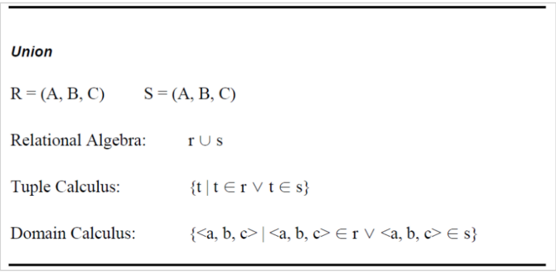
\includegraphics[width=0.8\textwidth]{../Lecture 4.2_artifacts/image_000029_4ae94d4a2cceb3e868774769502fc8082d42d3815444997958319488d1c8d013.png}
    \end{center}
\end{frame}

\begin{frame}{Equivalence of RA, TRC and DRC: Set Difference}
    \begin{center}
        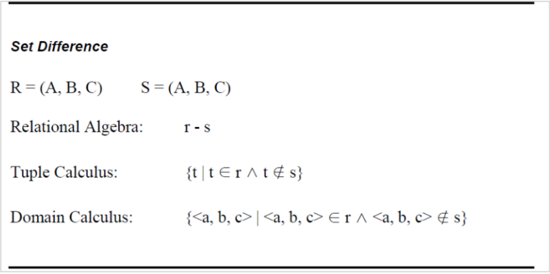
\includegraphics[width=0.8\textwidth]{../Lecture 4.2_artifacts/image_000031_2a1e07964144d3f09e74320a0515f603bb1e0c4dbd5153c3ba53c1a7b47abd77.png}
    \end{center}
\end{frame}

\begin{frame}{Equivalence of RA, TRC and DRC: Intersection}
\end{frame}

\begin{frame}{Equivalence of RA, TRC and DRC: Cartesian/Cross Product}
    \begin{center}
        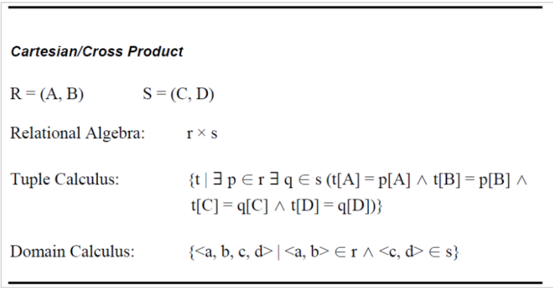
\includegraphics[width=0.8\textwidth]{../Lecture 4.2_artifacts/image_000034_f512c2bbf956f15f5c9fe525c70042cbc4e1ed493e16fc3b07752cb7f1d5595e.png}
    \end{center}
\end{frame}

\begin{frame}{Equivalence of RA, TRC and DRC: Natural Join}
    \begin{center}
        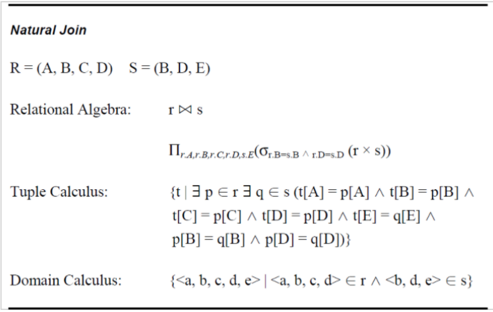
\includegraphics[width=0.8\textwidth]{../Lecture 4.2_artifacts/image_000036_113af1a861d1ffbdfc6f5c3fd057305501c8b54388224e3b5356428e5fb1f468.png}
    \end{center}
\end{frame}

\begin{frame}{Equivalence of RA, TRC and DRC: Division}
\end{frame}

\begin{frame}{Module Summary}
    \begin{itemize}
        \item Introduced tuple relational and domain relational calculus
        \item Illustrated equivalence of algebra and calculus
    \end{itemize}
    \vspace{2em}
    \begin{center}
    \small \textit{Slides used in this presentation are borrowed from \url{http://db-book.com/} with kind permission of the authors.} \\
    \small \textit{Edited and new slides are marked with 'PPD'.}
    \end{center}
\end{frame}

\end{document}
